% SDSS 2027 refereed abstract: two-page extended abstract, BLINDED (no author names).
% Draft, 23 November 2026. Before submitting, paste the text into the official SDSS LaTeX/Overleaf
% or Word template (sdss2020.sty) and check that it still fits on two pages.
\documentclass[10pt,twocolumn]{article}
\usepackage[letterpaper,margin=0.75in,columnsep=0.3in]{geometry}
\usepackage[T1]{fontenc}
\usepackage{mathptmx}
\usepackage{amsmath}
\usepackage{graphicx}
\usepackage{booktabs}
\usepackage{caption}
\captionsetup{font=small,labelfont=bf,skip=3pt}
\usepackage{titlesec}
\titleformat{\section}{\fontsize{12}{14}\bfseries}{\thesection}{0.5em}{}
\titlespacing*{\section}{0pt}{6pt}{3pt}
\setlength{\parskip}{2pt}
\pagestyle{empty}
\begin{document}
\twocolumn[{%
\begin{center}
{\fontsize{15}{18}\bfseries Weighted PageRank and Official Rankings in Tennis and Other Sports}\\[8pt]
{\fontsize{12}{14}\selectfont\bfseries Anonymous}\\[2pt]
{\small Affiliation withheld for review}\\[10pt]
\end{center}
\begin{minipage}{0.92\textwidth}\centering\small
\textbf{Abstract.} I compare official sports rankings with rankings computed by weighted PageRank on the network of match results, over five decades of professional tennis and in several other sports. I study how well correlated the two rankings are, which one better predicts the next season's matches, and what their differences reveal about each ranking rule.\\[3pt]
\textbf{Keywords:} PageRank; network science; sports rankings; tennis; prediction
\end{minipage}
\vspace{10pt}
}]

\section{Introduction}
Official sports rankings follow rules set by each sport's governing body. The ATP and WTA rankings in tennis add up points for the round a player reaches in each tournament, the FIFA men's ranking uses an Elo-type rating, and team sports use league tables. None of these looks directly at the whole network of results: who beat whom, and how strong those opponents were.

Network science offers such a view. If every season is a directed network in which each loser points to the winner, a competitor ranks highly by beating competitors who themselves rank highly, the idea behind PageRank \cite{brin}. Win-weighted PageRank has been applied to tennis before \cite{radicchi,dingle}. In this work I compare it systematically with the official rankings over five decades of men's and women's tennis and in five other competitions, and ask three questions: (1) how well correlated are the two rankings; (2) which one better predicts the next season's matches; and (3) where, and why, do they disagree?

\begin{figure*}[t]
\centering
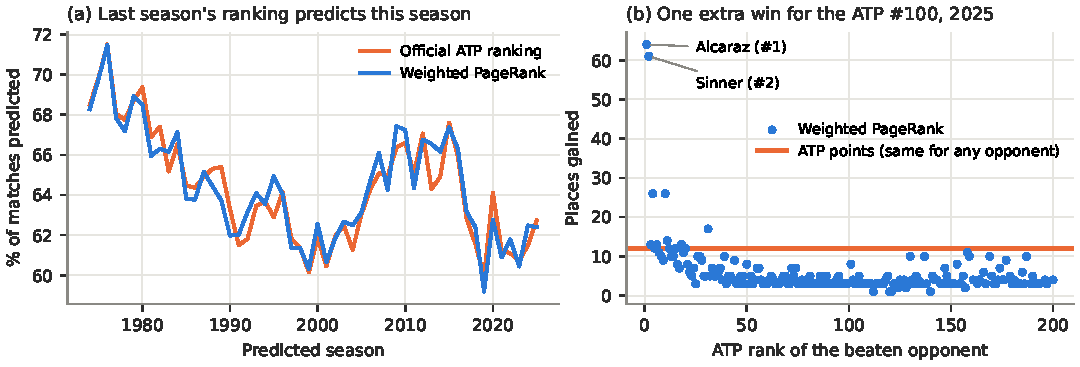
\includegraphics[width=0.9\textwidth]{figure.pdf}
\caption{(a) Share of each season's ATP matches whose winner was ranked higher at the end of the previous season, by the official ATP ranking and by weighted PageRank. (b) Places gained in the 2025 rankings by the ATP number 100 from one extra win, by the ATP rank of the beaten opponent; the orange line is the gain under ATP points, the same for every opponent.}
\label{fig:main}
\end{figure*}

\section{Data and Methods}
\textbf{Data.} Tennis: all tour-level main-draw matches and weekly rankings of the ATP (1973--2026) and the WTA (1984--2026) \cite{sackmann}, without Davis Cup, team exhibitions and walkovers. Other sports: international football between FIFA members (August 2018--November 2026) with the FIFA ranking of 18 July 2024; the Premier League, NBA and NHL (2024--25 and 2025--26) and the NFL (2024 and 2025) regular seasons.

\textbf{Network.} For each season, every competitor is a node and every match adds 1 to the weight $w_{ji}$ of the edge from the loser $j$ to the winner $i$ (a draw adds 0.5 in each direction).

\textbf{Weighted PageRank (WPR).} With $s_j=\sum_i w_{ji}$ the losses of $j$, $N$ the number of competitors and $d=0.85$,
\begin{equation*}
\mathrm{WPR}(i)=\frac{1-d}{N}+d\!\!\sum_{j:\,w_{ji}>0}\!\!\mathrm{WPR}(j)\,\frac{w_{ji}}{s_j}+\frac{d}{N}\!\!\sum_{j:\,s_j=0}\!\!\mathrm{WPR}(j),
\end{equation*}
computed by power iteration and checked against NetworkX.

\textbf{Correlation.} Spearman's $\rho$ between WPR and the official year-end ranking (the top 100 in tennis).

\textbf{Predictability.} Each ranking at the end of season $t$ predicts every match of season $t+1$ between two competitors it ranks: the higher-ranked one should win. A correct prediction scores 1, a wrong one 0, and the percentage of ones measures predictability. Because both rankings make the same prediction for about nine matches in ten, I also report how often WPR is right on the matches where they disagree (binomial test) and in how many seasons each ranking is ahead (Wilcoxon signed-rank test).

\textbf{Disagreements.} (a) A controlled experiment adds one win for the ATP number 100 over each opponent in the top 200 and recomputes both rankings. (b) For every top-100 player-season 2010--2025, the \emph{gain} is the ATP position minus the WPR position, related to the player's schedule and region.

\section{Preliminary Results}
\textbf{Correlation.} The two rankings are well correlated: mean Spearman $\rho$ for the top 100 is 0.885 for men and 0.907 for women, 0.88--0.96 in the four leagues and 0.95 in international football. It is lowest when the official ranking does not describe the season, as in 2020, when the ATP ranking was frozen (0.71).

\textbf{Predictability.} Over 52 men's seasons the two rankings predict equally well (Table~\ref{tab:pred}): 64.4\% against 64.5\%, and WPR is right in 50.5\% of the 14,153 matches where they disagree ($p=0.26$). The official ranking was usually better before 1990, when it averaged results per tournament; since 1991 WPR has been slightly ahead (21 of 35 seasons, 63.5\% against 63.1\%). For women the WTA ranking is slightly but consistently better (65.0\% against 64.5\%, 33 of 41 seasons). In the other sports, with one season each, the differences go both ways and none is large.

\begin{table}[t]
\centering\small
\caption{Percentage of next-season matches predicted correctly by last season's ranking.}
\label{tab:pred}
\setlength{\tabcolsep}{4pt}
\begin{tabular}{@{}lrrr@{}}
\toprule
Competition (predicted seasons) & Matches & Official & WPR \\
\midrule
Men's tennis (1974--2025) & 135,554 & 64.4 & 64.5 \\
Women's tennis (1985--2025) & 86,244 & 65.0 & 64.5 \\
International football$^{*}$ & 1,909 & 76.6 & 75.3 \\
NFL (2025) & 271 & 56.8 & 58.3 \\
NBA (2025--26) & 1,230 & 59.0 & 57.2 \\
NHL (2025--26) & 1,312 & 50.9 & 50.4 \\
Premier League (2025--26) & 203 & 58.4 & 59.6 \\
\bottomrule
\multicolumn{4}{@{}l@{}}{\footnotesize $^{*}$FIFA ranking of July 2024; matches to November 2026.}
\end{tabular}
\end{table}

\textbf{Disagreements.} Under ATP rules the points for a win do not depend on the opponent. Under WPR they do: one extra win over Carlos Alcaraz or Jannik Sinner lifts the 2025 ATP number 100 by 64 and 61 places, against 12 places under ATP points (Figure~\ref{fig:main}b). The value of a win follows the beaten player's score divided by his number of losses (Spearman 0.96), not his ATP rank (0.44). Across 1,598 top-100 player-seasons, WPR ranks lower the players with few tour-level matches (mean gain $-8.1$ places for 20 or fewer), those whose points come mostly from the biggest events ($-7.0$ when over 75\% of matches), and South American players ($-2.0$, $p=0.014$), whose ATP 250 events have weaker fields (median beaten player ranked 89, against 70 in Europe).


\section{Discussion}
A ranking built only from who beat whom is well correlated with the official rankings and predicts the next season about as well, so it is best used as a transparent check rather than a replacement. Its value lies in the disagreements, which show what each ranking rule rewards: deep runs at the biggest events, the number of tournaments entered, and the region where a player competes. Next steps are more seasons for the team sports, weights that let older matches count less, and sports without head-to-head matches, such as golf.

\small
\begin{thebibliography}{9}\setlength{\itemsep}{0pt}
\bibitem{brin} S. Brin and L. Page. The anatomy of a large-scale hypertextual Web search engine. \emph{Computer Networks and ISDN Systems}, 30:107--117, 1998.
\bibitem{radicchi} F. Radicchi. Who is the best player ever? A complex network analysis of the history of professional tennis. \emph{PLoS ONE}, 6(2):e17249, 2011.
\bibitem{dingle} N. Dingle, W. Knottenbelt and D. Spanias. On the (Page) ranking of professional tennis players. In \emph{Computer Performance Engineering}, LNCS 7587, 237--247. Springer, 2013.
\bibitem{sackmann} J. Sackmann. Tennis ATP and WTA match and ranking data. GitHub, 2026 (CC BY-NC-SA 4.0).
\end{thebibliography}
\end{document}
